The LHC is a $pp$ collider.
% Talk about the LHC being a hadron collider and the difficulties associated
% with it
Unlike electron, proton is a composite particle, made of $u, u, d$ quarks.
From the parton distribution functions of LHCb\footnote{
    Number density to find fraction of the momentum (denoted as $x$) at certain
    squared energy scale $Q^2$.
}, we see that there are plenty of other elementary particles, such as gluons,
that can participate in the collision.
These particles may carry varying portion of the total
momentum \cite{Ball:2014uwa}.

Effectively, partons, including gluons, are being collided.
Due to the unavoidable strong actions, many unwanted particles will be
generated---Comparing to \BaBar/, one notable addition of LHCb is the triggering
system, which is used to filter out uninteresting events, reducing the readout
rate \cite{LHCb:2008}.
Also, since we do not know the precise fraction of momentum carried by
interactive partons\footnote{
Again, these are characterized by parton distribution functions}, it is harder
to tell signal from normalization.

It is obvious that $e^- e^+$ colliders provide a \emph{much} cleaner background.
However, the LHC generates much more $b\bar{b}$\footnote{
    Note that this is \emph{not} necessarily \Y4S/.
} events compared to \BaBar/, due to a much larger cross section.
At \SI{13}{TeV}, the measured cross section at LHCb\footnote{
    For $2 < \eta < 5$ only, since this is the LHCb acceptance range.
} is $144 \pm 1 \pm 21$~\si{\mu b} \cite{Aaij:2016avz}.
% FIXME: Is the calculation for BaBar cross section legal?
Use the integrated luminosity and total number of $B\overline{B}$ events
contained in the on-resonance \Y4S/ sample, we compute the $b\bar{b}$ cross
section of \BaBar/ to be $\approx 1.09$~\si{nb}, which is much smaller than that
of the LHCb.

% Talk about subdetectors
LHCb, a single-arm spectrometer, is one of the four large experiments at the
LHC.
Its constituent subdetectors, from closest to farthest from the collision point,
are shown in \autoref{fig:lhcb_detector_view}:
The Vertex Locator (VELO) provides precise measurements of track coordinates
close to the collision point.
Two Ring Imaging Cerencov counters (RICH1, RICH2) provide particle
identification for charged particles over a wide range of momentum.
Tracker Turicensis (TT) and Inner Tracker (IT) provide additional tracking for
charged particles.
The Outer Tracker (OT) is used for tracking, as well as measures the momentum
of charged particles.
The calorimeters (ECAL and HCAL) have a first-level (L0) trigger to select
hadron, electron, and photon candidates based on their transverse momentum
$p_T$;
they also provide identification for the particles listed above;
finally, they provide energy and position measurements for these particles.
The Muon system (M1-5) is farthest from the collision point;
it provides L0 high $p_T$ muon trigger, and a high-level trigger (HLT) for muon
identification \cite{LHCb:2008}.

\begin{figure}[ht]
    \centering
    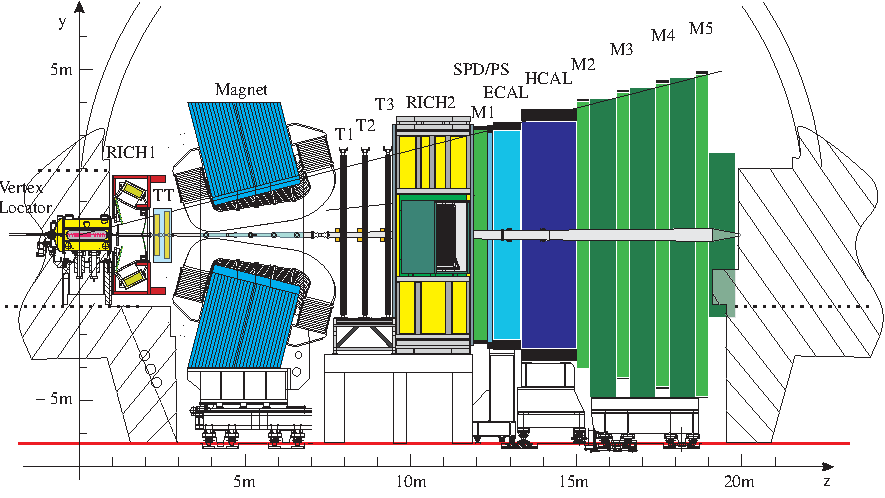
\includegraphics[width=0.7\textwidth]{figs/lhcb_detector_view.pdf}
    \caption{
        View of the LHCb detector.
        Vertex Locator (VELO) is closest to collision point.
    }
    \label{fig:lhcb_detector_view}
\end{figure}

% Talk about LHCb being forward-only
An interesting design choice is the geometry of the LHCb detector:
Instead of being a barrel $4\pi$ detector, it is forward-only.
This is because at high energies, $b\bar{b}$ is mostly produced in the forward
and backward direction.
The LHCb design is a very cost-effective way to construct a detector at the LHC
dedicated for $B$ physics \cite{LHCb:2008}.

% Talk about tracking
LHCb has a very good vertexing and tracking system, some of the subdetectors has
a better resolution, even compared to \BaBar/;
but its calorimeters are mediocre \cite{LHCb:2008,Guz:2017}, which makes the
reconstruction of charge-neutral particles, such as $\pi^0$, less precise.
This is why LHCb analyses typically focus on final states with charged particles
only, whereas \BaBar/ can afford to use final states with neutral particles.
We will come back to this point in the next section.

% Talk about run 1 and run 2 luminosity
LHCb collected data from 2010 to 2012 (Run 1), and 2015 to 2018 (Run 2).
An incomplete integrated luminosity (summing from 2010 to 2017) is
\SI{6.829}{fb^{-1}} \cite{LHCb-Facts:2019}.

% Talk about LS2 upgrade and LHCb's future
%Currently, LHCb is shut down for an upgrade.
%We, the University of Maryland group, are actively participating in the upgrade.
%Specifically, we are designing data transmission system as well as power
%delivery system for the Upstream Tracker (UT) upgrade, which will replace the TT
%in Run 3.

%The current TT system limits the readout rate to \SI{1}{MHz}, due to the L0
%hardware trigger.
%The updated UT will have a \SI{40}{MHz} rate, which will make a fully
%software-based trigger possible \cite{LHCbCollaboration:2014tuj}.
%Another benefit is to reduce ghost tracks\footnote{
    %Ghost tracks are formed by linking VELO tracks with the wrong downstream
    %tracks.
%} by providing additional measurements between VELO and downstream trackers
%(currently IT, will be replaced by SciFi tracker) \cite{Parker:2017}.
